\documentclass[UTF8,fontset=none,zihao=-4,a4paper]{ctexart}
\usepackage[margin=25mm]{geometry}
\usepackage{fontspec}
\setmainfont{NimbusRoman-Regular.otf}[
  BoldFont=NimbusRoman-Bold.otf, ItalicFont=NimbusRoman-Italic.otf,
  BoldItalicFont=NimbusRoman-BoldItalic.otf]
\setCJKmainfont{NotoSerifCJK-Regular.ttc}[
  FontIndex=2, BoldFont=NotoSerifCJK-Bold.ttc,
  ItalicFont=NotoSerifCJK-Regular.ttc, SlantedFont=NotoSerifCJK-Regular.ttc]
\setCJKsansfont{NotoSansCJK-Regular.ttc}[FontIndex=2,BoldFont=NotoSansCJK-Bold.ttc]
\usepackage{amsmath,amssymb,booktabs,graphicx,xcolor}
\usepackage{caption}
\usepackage[unicode,hidelinks]{hyperref}
\usepackage{url}

\definecolor{sectionink}{HTML}{183B50}
\ctexset{
  section={format=\Large\bfseries\color{sectionink},number=\arabic{section}},
  subsection={format=\normalsize\bfseries,number=\arabic{section}.\arabic{subsection}}
}
\captionsetup{font=small,labelfont=bf,justification=centering}
\hypersetup{
  pdftitle={俄罗斯方块 AI 的长期生存与得分评测},
  pdfsubject={Tetris AI Benchmark 技术报告},
  pdfkeywords={Tetris, reinforcement learning, imitation learning, right censoring}
}
\urlstyle{same}
\renewcommand{\arraystretch}{1.13}
\setlength{\parindent}{2em}
\setlength{\textfloatsep}{1.1em plus .3em minus .2em}
\setlength{\intextsep}{1.0em plus .3em minus .2em}
\raggedbottom
\pagestyle{plain}
\newcommand{\repo}{\href{https://github.com/u-wyh/tetris-ai-benchmark}{Tetris AI Benchmark}}
\newcommand{\1}{\mathbf{1}}

% Generated from episodes.csv by analysis.py.
\newcommand{\ResultsShort}{%
A1 & BC Champion & 97\,861 & 100\,000 & 31/32 & 81.06 & 0.04 \\
 & Hybrid B12 & 71\,941 & 11\,080 & 19/32 & 102.91 & 91.08 \\
 & PPO 30M & 61\,823 & 13\,225 & 9/32 & 78.22 & 93.16 \\
\midrule
A2 & BC Champion & 100\,000 & 100\,000 & 32/32 & 83.35 & 0.03 \\
 & Hybrid B12 & 79\,743 & 15\,738 & 21/32 & 117.74 & 90.98 \\
 & PPO 30M & 71\,688 & 17\,395 & 16/32 & 100.64 & 93.04 \\
}

% Generated from episodes.csv by analysis.py.
\newcommand{\ResultsLong}{%
B & BC Champion & 2\,365\,529 & 1\,162\,680 & 5/8 & 55\,003.47 & 0.03 \\
 & V2 Hold-only & 1\,436\,759 & 130\,038 & 2/8 & 28\,414.52 & 0.03 \\
 & Hybrid B12 & 194\,285 & 36\,834 & 0/8 & 897.82 & 91.10 \\
 & PPO 30M & 100\,672 & 14\,084 & 0/8 & 329.44 & 93.10 \\
}

% Generated from episodes.csv by analysis.py.
\newcommand{\ResultsEffects}{%
A1 & BC Champion $-$ PPO 30M & 存活（千块） & 36.04 & [22.96, 48.88] \\
 & Hybrid B12 $-$ PPO 30M & 存活（千块） & 10.12 & [-8.72, 28.34] \\
 & Hybrid B12 $-$ PPO 30M & 总分（亿） & 24.69 & [-10.19, 58.82] \\
 & Hybrid B12 $-$ BC Champion & 总分（亿） & 21.85 & [-1.64, 44.16] \\
\midrule
A2 & BC Champion $-$ PPO 30M & 存活（千块） & 28.31 & [16.48, 40.66] \\
 & Hybrid B12 $-$ PPO 30M & 存活（千块） & 8.06 & [-10.17, 25.76] \\
 & Hybrid B12 $-$ PPO 30M & 总分（亿） & 17.10 & [-17.63, 50.78] \\
 & Hybrid B12 $-$ BC Champion & 总分（亿） & 34.39 & [11.87, 55.10] \\
\midrule
B & BC Champion $-$ V2 Hold-only & 存活（千块） & 928.77 & [238.16, 1\,717.42] \\
}


\begin{document}

\begin{center}
  {\small\sffamily Tetris AI Benchmark 技术报告\par}
  \vspace{0.6em}
  {\zihao{2}\bfseries 俄罗斯方块 AI 的长期生存与得分评测\par}
  \vspace{0.35em}
  {\zihao{4} 启发式、强化学习、行为克隆与混合策略的配对比较\par}
  \vspace{0.65em}
  {\large\bfseries Evaluating Long-Horizon Survival and Score in Tetris AI\par}
  \vspace{0.2em}
  {A Paired Comparison of Heuristics, Reinforcement Learning,\par
   Behavioral Cloning, and Hybrid Control\par}
  \vspace{0.55em}
  {\small 2026 年 11 月 23 日\par}
\end{center}

\noindent\textbf{摘\quad 要}\quad
俄罗斯方块策略的累计得分同时受到消行方式、等级与对局长度影响，固定步数的评测还会截断长寿命策略。本文基于统一的公开观察、合法落点和计分规则，对启发式 V2 Hold-only、带动作掩码的 PPO、行为克隆（BC）和风险拦截混合策略 B12 进行回顾性配对评测。本文从既有实验中提取 224 局逐局记录。两批各 32 个独立种子的 10 万块评测中，BC 分别有 31 局和 32 局达到上限，B12 的平均总分分别为 102.91 亿和 117.74 亿，均为三种受测策略中最高。在另 8 个种子、每局上限 300 万块的评测中，BC、V2、B12 和 PPO 的截断平均存活分别为 236.55 万、143.68 万、19.43 万和 10.07 万块。BC 对 V2 的平均优势约 92.88 万块，配对 Bootstrap 95\% 区间为 23.82 万至 171.74 万块。结果表明，报告存活分布、触顶比例与得分，可以揭示单一指标难以区分的策略特性。

\smallskip
\noindent\textbf{关键词}\quad 俄罗斯方块，强化学习，行为克隆，配对评测，右截断

\medskip
{\small
\noindent\textbf{Abstract.}\enspace
Cumulative Tetris scores depend on line-clear patterns, level progression, and episode length. Evaluation caps also censor long-lived policies. Under a common public observation, legal-placement rule, and scoring system, we retrospectively compare a Hold-only heuristic, masked PPO, behavioral cloning (BC), and a risk-gated hybrid (B12) using 224 archived episodes. Across two independent 32-seed cohorts capped at 100,000 pieces, BC reached the cap in 31 and 32 episodes, respectively. B12 attained the highest mean total score among the three evaluated policies in both cohorts, at 10.29 and 11.77 billion points. In a separate eight-seed cohort capped at three million pieces, restricted mean survival was 2.366 million for BC, 1.437 million for the heuristic, 0.194 million for B12, and 0.101 million for PPO. The mean paired BC--heuristic difference was 0.929 million pieces, with a descriptive 95\% bootstrap interval of [0.238, 1.717] million. Reporting capped survival and scoring outcomes together reveals how policy rankings depend on the evaluation objective and protocol.
\par\smallskip
\noindent\textbf{Keywords.}\enspace Tetris, reinforcement learning, behavioral cloning, paired evaluation, right censoring\par}

\section{引言}

俄罗斯方块要求策略在连续出现的方块序列上反复选择落点。消行会降低堆叠高度并获得分数，保留可供四消的结构也可能增加未来的布局约束。某些破坏性局面很少出现，却足以决定长局的尾部风险。因此，短局均分、消行方式和长程生存都值得独立测量。

以往研究在俄罗斯方块上检验了手工棋盘特征、交叉熵优化和近似策略迭代等方法\cite{thiery2009,gabillon2013}。跨实现比较受棋盘、动作可达性、方块生成及评分定义影响。本文关注同一实现内的策略比较，通过项目的 JavaScript 和 Python 规则一致性测试固定评测语义\cite{rules}。在该规则下，考察三个问题：（1）两批独立种子上的生存和得分排序是否一致；（2）更高上限的长局能否区分经常触顶的模仿学习策略与其启发式教师；（3）保留 PPO 四消行为的风险拦截在不同指标上有何权衡。

\section{基准环境与策略}

\subsection{公开观察、动作与计分}

棋盘为 20 行、10 列，环境按七块一袋的随机机制生成方块，每袋包含七种方块各一枚。策略可见棋盘、当前方块、暂存（Hold）及其可用状态、后续三个方块和公开计分状态。种子、随机数发生器状态、袋中剩余顺序和更远的方块属于环境内部状态。

动作对应一个完整落点，编码为
\[
  \mathcal{A} = \{0,1\}\times\{0,1,2,3\}\times\{0,\ldots,9\}
  \times\{-3,\ldots,19\}.
\]
四个分量依次表示是否使用 Hold、旋转状态和最终占据格的左上坐标。每个状态的合法集合 $\mathcal{A}(s)\subseteq\mathcal{A}$ 由广度优先搜索产生。搜索使用左移、右移、顺时针旋转、下移及旋转踢墙规则，并对同一 Hold 分支中的等价占据格仅保留最小动作编号。动作掩码刻画机械可达性。人工模式的落地计时独立于 AI 的逐块落点语义\cite{rules}。

单消、双消、三消、四消分别给出 $100, 300, 500, 800$ 乘以消行前等级的基础分，另计规则规定的下落分。每累计消除 10 行升一级，Benchmark v1.0 的计分项不含 T-Spin、连击、背靠背及全清奖励。训练奖励和正式累计分数分别记录。

\subsection{启发式与候选评分网络}

\textbf{V2 Hold-only。} 在允许使用 Hold 的合法落点中，模拟一步落子并按消行数、总高度、洞、压洞、崎岖度、井、行列转换和顶部风险等特征的线性组合选点。一步模拟检测公开信息可判定的终止条件。V2 是长局对照策略，也是行为克隆的示范教师。

\textbf{PPO 30M。} 策略采用近端策略优化（PPO）\cite{schulman2017}和无效动作掩码\cite{huang2022}。候选评分网络将 237 维公开状态向量 $s$ 和每个合法动作对应的 16 维候选特征 $f(s,a)$ 分别编码，将两个 64 维嵌入拼接，再用共享评分头产生 logit $z_\theta(s,a)$。候选特征包括消行、堆叠高度、洞和表面几何等落子后统计量。价值网络只使用公开状态向量。策略分布为
\begin{equation}
   \pi_\theta(a\mid s)=
   \frac{\1\{a\in\mathcal{A}(s)\}\exp z_\theta(s,a)}
        {\sum_{b\in\mathcal{A}(s)}\exp z_\theta(s,b)} .
   \label{eq:masked}
\end{equation}
冻结模型累计训练 30\,003\,200 个环境步骤。训练使用 8 个并行环境（种子 42--49），学习率 $3\times10^{-4}$，折扣 $\gamma=0.995$，GAE 系数 $\lambda=0.95$，PPO 截断参数 $0.2$。每个环境采样 512 步后更新，小批量 256，每次更新训练 5 轮。每步基础奖励为 $0.001$，按消除 $0$ 至 $4$ 行附加 $(0,1,3,5,8)$，实际终止扣 2。评测采用掩码内确定性贪心选择。

\textbf{BC Champion。} 在 20M PPO 检查点上以 V2 Hold-only 的合法动作作为标签，最小化 $-\log\pi_\theta(a_{\mathrm{V2}}\mid s)$，只更新状态编码器、候选编码器和评分头。示范数据共 214\,809 条，训练和验证按完整对局种子划分，分别使用 100 个和 8 个种子。批量大小为 16，Adam 学习率 $10^{-4}$，冻结版本取第 3 轮\cite{bcdata}。行为克隆在专家轨迹上学习，在自身轨迹上可能遇到分布偏移\cite{ross2011}，因此本文以整局指标评估该检查点。

\subsection{风险拦截混合策略}

混合策略 B12 每步同时计算 PPO 和 BC 的贪心落点。令 $D$ 表示落锁出界，$C$ 为顶部四行中间四列的占据格数，$H$ 为落子并消行后的最大列高，$H_0$ 为落子前的最大列高，$N$ 为新增洞数，$U$ 为落子后的表面崎岖度。实现使用的一步风险为
\begin{equation}
    R = 10^6D + 10^3C + 100[H-11]_+ + 35N + 12[H-H_0]_+ + 2U,
    \qquad [x]_+=\max(0,x).
    \label{eq:risk}
\end{equation}
PPO 候选出现落锁出界、顶部中央占据，或落子后列高达到 12 且高度上升或新增洞时触发比较。只有 BC 候选无落锁出界、风险至少低 100、落子后高度和顶部中央占据均不超过 PPO 时，才采用 BC 落点。其他状态执行 PPO 落点。两套网络参数冻结，风险拦截在推理时计算\cite{hybrid}。

\section{实验设计与统计量}

\subsection{固定种子和预算}

表~\ref{tab:protocol}列出三批配对协议。同一协议中，各受测策略使用相同种子和每局方块上限。A1 与 A2 分别来自两次独立确认实验\cite{aone,atwo}。本文提取两个协议共有的 BC、B12 和 PPO 冻结基线。协议 B 是单独的长局对照，包含 V2。同一批种子内做策略配对，三批分别报告。各协议使用同一对冻结的 PPO 与 BC 权重，B12 复用这两套权重。B 使用公开状态的加速合法落点实现，记录中有 3 局 PPO 由原 BFS 的同种子结果按哈希导入\cite{longcode}。

\begin{table}[htbp]
\centering
\caption{纳入分析的配对评测协议}
\label{tab:protocol}
\small
\begin{tabular}{llrrl}
\toprule
协议 & 种子范围 & 每种策略局数 & 每局上限（块） & 纳入策略 \\
\midrule
A1 & 1421000--1421031 & 32 & 100\,000 & BC、B12、PPO \\
A2 & 710100--710131 & 32 & 100\,000 & BC、B12、PPO \\
B  & 1400000--1400007 & 8  & 3\,000\,000 & BC、V2、B12、PPO \\
\bottomrule
\end{tabular}
\end{table}

\subsection{生存、总分与不确定性}

令 $T_i$ 为种子 $i$ 下的终止块数，$\tau$ 为预算，$X_i=\min(T_i,\tau)$ 为观测块数。到达上限且仍在运行的局计为右截断。由于协议内使用共同观测上限，$\bar X_\tau=n^{-1}\sum_i X_i$ 估计该上限内的限制平均生存。P10 为 $X_i$ 的第 10 百分位，按相邻次序统计量线性插值。图中以 $n^{-1}\sum_i\1\{X_i\ge t\}$ 表示达到阈值 $t$ 的样本比例。曲线在 $\tau$ 处结束。

每局总分为最后计分状态中的正式累计分，反映生存时长、等级和消行结构的联合作用。四消占比为所有四消事件数除以至少消一行的落子事件总数。该比例以事件数加权。总分表用于比较同协议下的实际结果。得分效率需要在共同对局长度上另行定义。

对每个比较，先按种子求策略差，再以种子为单位有放回地重抽 $n$ 对，重复 20\,000 次。以重采样均值的 2.5\% 和 97.5\% 分位点给出配对 Bootstrap 区间。本文为回顾性分析，区间用于描述样本不确定性，未做多重比较校正。B 组的 8 个种子尤其限制了推断精度。

\section{实验结果}

\subsection{两批 10 万块评测}

表~\ref{tab:short}显示，在 A1 与 A2 中，截断平均生存均按 BC、B12、PPO 排列，平均总分均以 B12 最高。BC 在 64 局中有 63 局触顶。B12 的四消事件比例约为 91\%，接近 PPO 的 93\%。B12 的生存 P10 在两批均低于 PPO，说明其平均生存和触顶数的提升可与部分种子的更短生存同时出现。

\begin{table}[htbp]
\centering
\caption{两批 10 万块评测结果}
\label{tab:short}
\small
\begin{tabular}{llrrrrr}
\toprule
协议 & 策略 & 平均存活 & P10（块） & 触顶 & 平均总分（亿） & 四消（\%） \\
\midrule
\ResultsShort
\bottomrule
\end{tabular}
\end{table}

\subsection{300 万块长局}

在协议 B 中，BC 的限制平均生存为 V2 的约 1.65 倍，为 PPO 的约 23.5 倍。BC 与 V2 分别有 5 局和 2 局触顶，实际终止块数在触顶局上未知。B12 平均存活 194\,285 块，超过同批 PPO 的 100\,672 块；两种策略在该批均于预算内终止。BC 的平均总分也高于其他三种策略，体现了该预算下累计得分随长局和等级增长的变化。图~\ref{fig:survival}展示三个协议的阈值达成比例。

\begin{table}[htbp]
\centering
\caption{300 万块长局评测结果}
\label{tab:long}
\small
\begin{tabular}{llrrrrr}
\toprule
协议 & 策略 & 平均存活 & P10（块） & 触顶 & 平均总分（亿） & 四消（\%） \\
\midrule
\ResultsLong
\bottomrule
\end{tabular}
\end{table}

\begin{figure}[htbp]
\centering
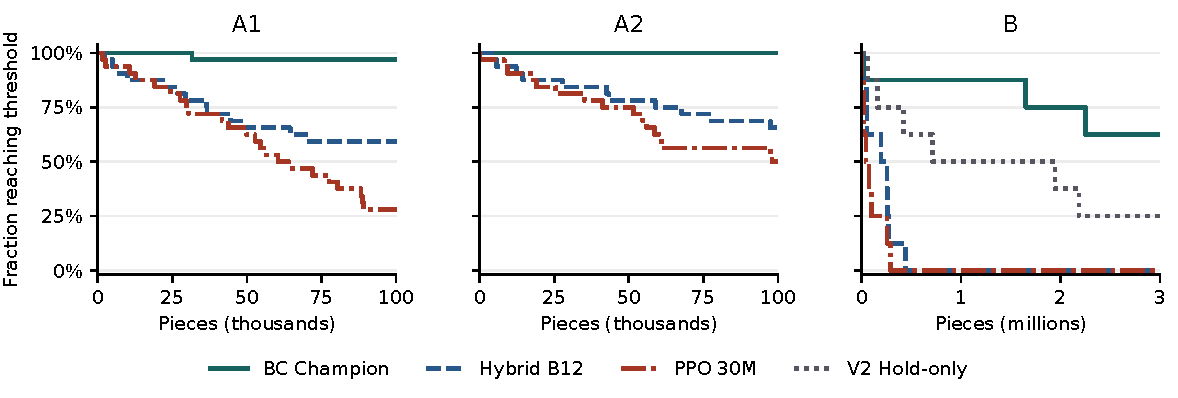
\includegraphics[width=\linewidth]{survival.pdf}
\caption{各协议内达到指定方块数的对局比例。A1、A2 横轴以千块为单位，B 以百万块为单位。最右端是评测预算，曲线不向预算外延伸。}
\label{fig:survival}
\end{figure}

\subsection{配对差及其不确定性}

表~\ref{tab:effects}给出种子配对结果。BC 相对 PPO 的限制平均生存差在两组方向一致，其 95\% 区间均位于零以上。B12 相对 PPO 的平均生存和平均总分在两组的点估计均为正，但区间均跨零。对 B 组，BC 相对 V2 的限制平均存活差为 92.88 万块，区间为 23.82 万至 171.74 万块。该区间位于零以上，但较宽，且仅反映由 8 个种子估计的变异。

\begin{table}[htbp]
\centering
\caption{平均配对差与 95\% Bootstrap 区间}
\label{tab:effects}
\small
\begin{tabular}{lllrr}
\toprule
协议 & 配对差（前者减后者） & 指标 & 均值 & 95\% 区间 \\
\midrule
\ResultsEffects
\bottomrule
\end{tabular}
\end{table}

\section{讨论}

\textbf{生存与得分。} 在两批 10 万块对照中，模仿学习策略频繁触顶，B12 保留了 PPO 的高四消频率并取得较高总分。B12 的低分位和宽配对区间表明，按平均总分选择策略仍会接受一定的短局风险。300 万块协议更适合观察 BC 与 V2 的长程差异，但其种子数量较少。两组名次变化反映了种子集和评测预算的共同变化。

\textbf{公开后续方块规划。} 项目另行评测了一种使用公开 Next 3 的有限步规划器。在单独的 32 种子、10 万块上限确认组中，规划器与 BC 的触顶数为 31 和 32。按同种子双方共同存活长度比较，规划器得分比 BC 高 10.54\%，配对 Bootstrap 95\% 区间为 $[10.43\%,10.64\%]$\cite{lookahead}。该组使用独立协议，证据支持规划器在这批对局的共同长度内提高得分。其长局延伸评测中途停止，这里仅报告独立确认组的结果。

\textbf{适用边界。} 结果对应一个固定的规则实现、确定性推理和少量冻结模型，区间估计的是种子差异，未覆盖重新训练的变异。PPO 与 BC 的目标、初始化和训练数据不同，因此当前对照无法单独估计某一训练选择的因果效果。受右截断限制，本文的寿命结论均以对应预算为界。协议和模型在其他俄罗斯方块实现中的表现需在相应规则下另行评测。

\section{结论}

在统一合法落点和计分规则下，BC Champion 在两批 10 万块确认组与 300 万块长局中的限制平均生存均居首，Hybrid B12 则在两批 10 万块确认组中取得最高平均总分，并保留较高四消比例。BC 相对传统 V2 的长局均值优势仍有较大不确定性。对这类长程控制任务，配对种子、明确的评测上限和对生存尾部的报告，是解释得分结果和跨策略比较的必要条件。

\section*{数据与代码可用性}

本文的 224 局汇总逐局数据、统计脚本、图表及排版源文件与 PDF 随 \repo{} 同目录归档。逐局 CSV 保留原始结果文件的 SHA-256 和终止标记，可独立重算本文主表和生存曲线。原始轨迹和神经网络权重存放于项目本地运行目录，仓库提供权重哈希及代码版本，用于在取得相同权重后核验和复跑。实验与生成说明见
\href{https://github.com/u-wyh/tetris-ai-benchmark/tree/codex/hardware-safe-autonomy/reports/paper}{论文目录}。

\begin{thebibliography}{10}
\small

\bibitem{thiery2009}
Thiery C, Scherrer B.
Improvements on Learning Tetris with Cross Entropy.
\textit{ICGA Journal}, 2009, 32(1): 23--33.
\href{https://doi.org/10.3233/ICG-2009-32104}{doi:10.3233/ICG-2009-32104}.

\bibitem{gabillon2013}
Gabillon V, Ghavamzadeh M, Scherrer B.
Approximate Dynamic Programming Finally Performs Well in the Game of Tetris.
\textit{Advances in Neural Information Processing Systems}, 2013, 26.
\href{https://papers.neurips.cc/paper_files/paper/2013/hash/7504adad8bb96320eb3afdd4df6e1f60-Abstract.html}{论文页面}.

\bibitem{rules}
Tetris AI Benchmark.
Benchmark v1.0 计分、公开观察与合法落点规则，2026.
\href{https://github.com/u-wyh/tetris-ai-benchmark/blob/c1395ccd7ecc0908ddf5289d1887978e1b87c0b5/tetris-game/README.md}{固定提交中的规则说明}.

\bibitem{schulman2017}
Schulman J, Wolski F, Dhariwal P, Radford A, Klimov O.
Proximal Policy Optimization Algorithms.
\textit{arXiv preprint}, 2017.
\href{https://arxiv.org/abs/1707.06347}{arXiv:1707.06347}.

\bibitem{huang2022}
Huang S, Onta\~n\'on S.
A Closer Look at Invalid Action Masking in Policy Gradient Algorithms.
\textit{Proceedings of the International Florida Artificial Intelligence Research Society Conference}, 2022, 35.
\href{https://doi.org/10.32473/flairs.v35i.130584}{doi:10.32473/flairs.v35i.130584}.

\bibitem{bcdata}
Tetris AI Benchmark.
Candidate Imitation Learning: V2 Hold, Behavioral Cloning, and PPO，2026.
\href{https://github.com/u-wyh/tetris-ai-benchmark/blob/c1395ccd7ecc0908ddf5289d1887978e1b87c0b5/reports/experiments/candidate_imitation_learning.md}{示范数据与训练报告}.

\bibitem{ross2011}
Ross S, Gordon G, Bagnell D.
A Reduction of Imitation Learning and Structured Prediction to No-Regret Online Learning.
\textit{Proceedings of the 14th International Conference on Artificial Intelligence and Statistics}, 2011, 15: 627--635.
\href{https://proceedings.mlr.press/v15/ross11a.html}{PMLR 论文页面}.

\bibitem{hybrid}
Tetris AI Benchmark.
PPO 30M + BC 双策略融合实验，2026.
\href{https://github.com/u-wyh/tetris-ai-benchmark/blob/c1395ccd7ecc0908ddf5289d1887978e1b87c0b5/reports/experiments/candidate_ppo30m_bc_hybrid.md}{实验报告}.

\bibitem{aone}
Tetris AI Benchmark.
PPO 30M 新候选独立 100K 确认，2026.
\href{https://github.com/u-wyh/tetris-ai-benchmark/blob/c1395ccd7ecc0908ddf5289d1887978e1b87c0b5/reports/experiments/ppo30m_independent_confirmation.md}{A1 评测报告}.

\bibitem{atwo}
Tetris AI Benchmark.
Hybrid V2 统一对照，2026.
\href{https://github.com/u-wyh/tetris-ai-benchmark/blob/c1395ccd7ecc0908ddf5289d1887978e1b87c0b5/reports/experiments/hybrid_v2_comparison.md}{A2 评测报告}.

\bibitem{longcode}
Tetris AI Benchmark.
三百万块配对评测，2026.
\href{https://github.com/u-wyh/tetris-ai-benchmark/blob/c1395ccd7ecc0908ddf5289d1887978e1b87c0b5/training/evaluation/post_curriculum_3m.py}{评测代码}，
\href{https://github.com/u-wyh/tetris-ai-benchmark/blob/c1395ccd7ecc0908ddf5289d1887978e1b87c0b5/reports/experiments/model_leaderboard.md}{结果索引}.

\bibitem{lookahead}
Tetris AI Benchmark.
公开 Next3 有限步规划：最终结论，2026.
\href{https://github.com/u-wyh/tetris-ai-benchmark/blob/a3bfc0276f338b3af8978c73bba86f8ef3129e69/reports/experiments/model_based_planning_final.md}{独立确认报告}.

\end{thebibliography}
\end{document}
